\subsubsection{Controlled assistant roles}
The research assistant uses three logical roles within one controlled workflow: an \textbf{event research agent} retrieves relevant events from the prediction market and creates event-to-asset mappings; an \textbf{analysis coordinator} requests and performs approved calculations; and an \textbf{explanation agent} presents results in context and answer user's questions.

For ``How could the next rate decision affect my SPY and MSFT exposure?'', the assistant resolves the assets, horizon and analysis time. It retrieves an eligible event and proposes an event-to-asset explanation, but numerical responses must come from historical estimates or reviewed stress assumptions. 

\subsubsection{Guided research journey and interface}
A user selects an asset or hypothetical portfolio and chooses how far ahead to examine risk. EventLens presents relevant events, compares market probabilities with experimental wallet-informed estimates, and lets the user inspect wallet activity before exploring scenarios. The assistant explains the evidence, and saved reports preserve the analysis.

For example, a user researching SPY over five trading days could inspect an upcoming rate decision, identify which tracked wallets are increasing YES or NO exposure, and compare the resulting risk scenarios. An incompatible announcement horizon or unsupported asset-response estimate will be explained before the affected calculation is withheld.

\begin{figure}[H]
\centering
\begin{tikzpicture}[x=1cm,y=1cm,
 actor/.style={flowbox,text width=2.15cm,minimum height=0.78cm,font=\scriptsize\sffamily},
 usecase/.style={draw=line,fill=pale,ellipse,align=center,text width=5.55cm,
  minimum height=0.68cm,font=\scriptsize\sffamily,inner sep=3pt},
 association/.style={draw=muted,line width=0.65pt}]
\draw[line,rounded corners=2pt] (2.7,0.55) rectangle (11.0,-5.55);
\node[anchor=north west,font=\scriptsize\bfseries\sffamily] at (2.9,0.4) {EventLens};

\node[actor] (investor) at (0.9,-1.05) {Retail investor};
\node[actor] (professional) at (12.45,-2.9) {Finance\\professional};
\node[actor] (researcher) at (0.9,-4.65) {Researcher or\\evaluator};

\node[usecase] (browse) at (6.85,-0.6) {Browse \textbf{Overview}, \textbf{Watchlist}\\and \textbf{Events}};
\node[usecase] (ask) at (6.85,-1.5) {Ask the \textbf{Research assistant}};
\node[usecase] (compareprob) at (6.85,-2.4) {Compare \textbf{Market probability}\\and \textbf{Adjusted estimate}};
\node[usecase] (scenario) at (6.85,-3.35) {Run \textbf{Portfolio scenario analysis}\\and \textbf{Compare allocation}};
\node[usecase] (wallet) at (6.85,-4.25) {Review \textbf{Wallet evidence} and assumptions};
\node[usecase] (inspect) at (6.85,-5.05) {\textbf{Inspect evidence} and \textbf{Save report}};

\draw[association] (investor.east)--(browse.west);
\draw[association] (investor.east)--(ask.west);
\draw[association] (professional.west)--(compareprob.east);
\draw[association] (professional.west)--(scenario.east);
\draw[association] (professional.west)--(11.2,-2.9)--(11.2,-0.72)--([yshift=-1mm]browse.east);
\draw[association] (11.2,-2.9)--(11.2,-4.13)--([yshift=1mm]wallet.east);
\draw[association] (researcher.east)--(2.3,-4.65)--(2.3,-0.48)--([yshift=1mm]browse.west);
\draw[association] (2.3,-1.42)--([yshift=1mm]ask.west);
\draw[association] (researcher.east)--([yshift=-1mm]wallet.west);
\draw[association] (researcher.east)--(inspect.west);
\end{tikzpicture}
\caption{Representative use cases by user context. Associations show common entry points; supported functions are not exclusive to one role.}
\label{fig:user-use-cases}
\end{figure}

\subsubsection{Smart-wallet tracking and evidence inspection}
Users can browse wallets in covered events, filter by history and activity, and follow public addresses without connecting a wallet. Profiles show earlier resolved-event decisions, entry prices, subsequent price movements, reconstructed positions and an activity timeline. A provisional ``smart'' label denotes historically informative behaviour and is supported by a dated score, sample size and coverage assessment.

\clearpage
\subsubsection{Concept screens}
Figures~\ref{fig:overview-ui} and~\ref{fig:scenario-ui} illustrate the intended layout. They are conceptual interface images. Values are illustrative and do not represent research results.

The \textbf{Overview} screen combines the \textbf{Watchlist} with the selected event's \textbf{Market probability}, \textbf{Adjusted estimate}, \textbf{Evidence} status and \textbf{Probability history}. The \textbf{Research assistant} answers contextual questions and links to the \textbf{Probability run} and \textbf{Wallet evidence}. The \textbf{Events} and \textbf{Saved research} navigation items lead to detailed event review and preserved analyses.

The \textbf{Scenarios} screen is headed \textbf{Portfolio scenario analysis}. Users enter a \textbf{Paper portfolio}, select \textbf{Run scenario}, and review \textbf{95\% VaR}, \textbf{95\% expected shortfall} and \textbf{Event probability}. They can then choose \textbf{Compare allocation}, \textbf{Inspect evidence} or \textbf{Save report}. Inputs and results remain hypothetical and do not place orders.
\begin{figure}[H]
\centering
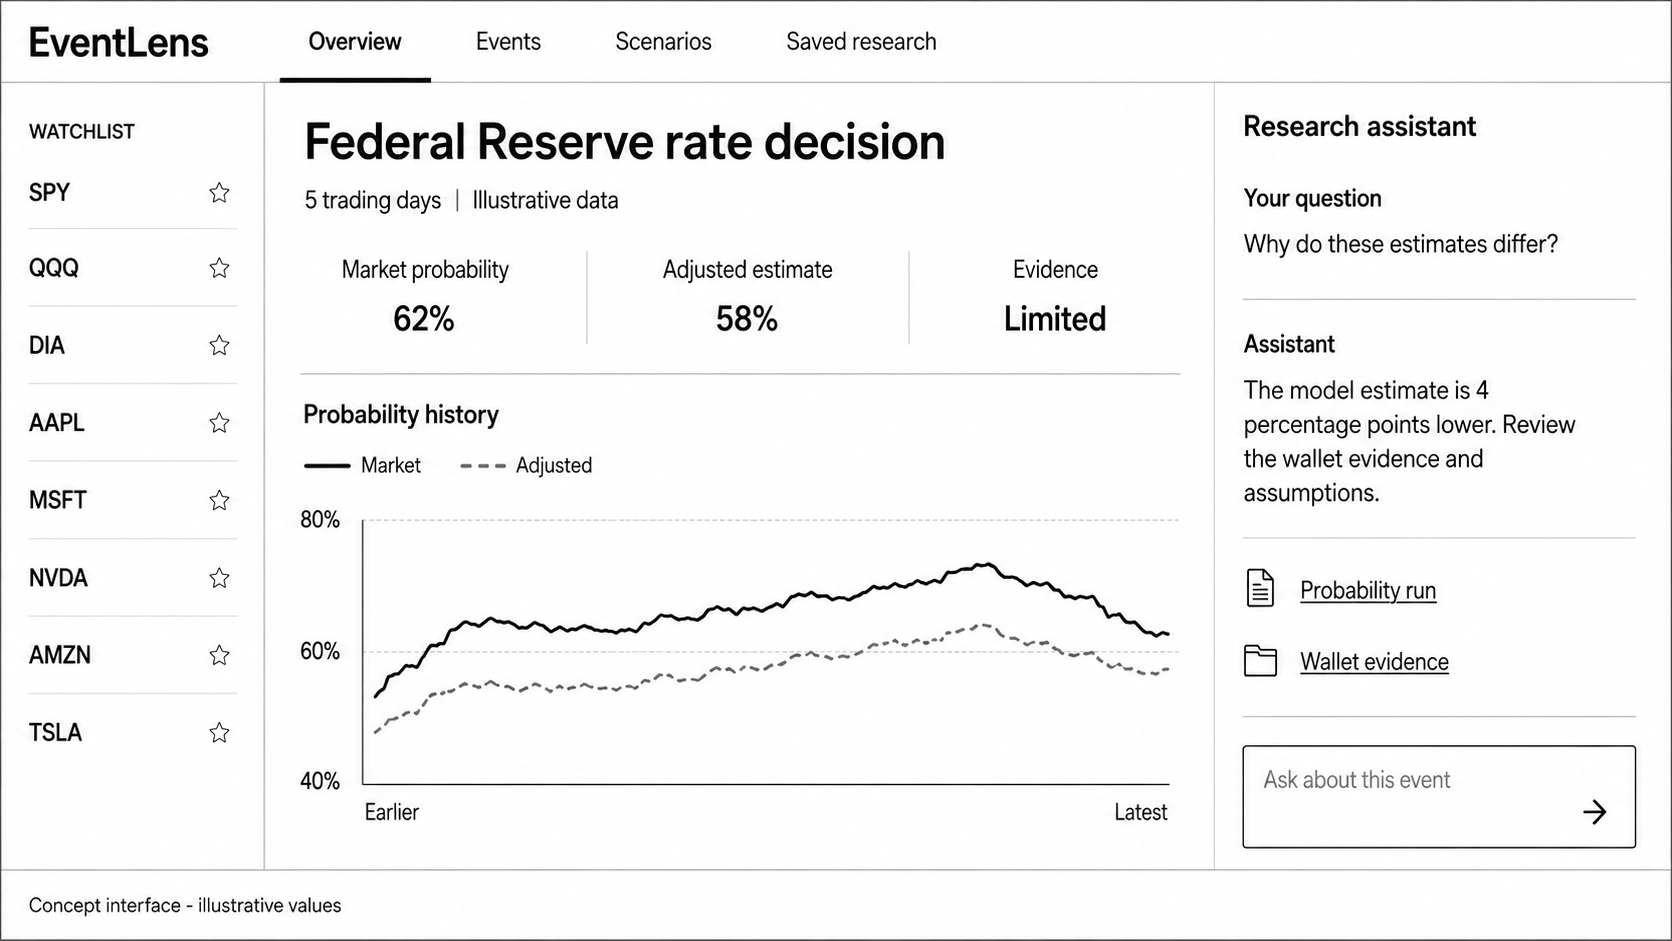
\includegraphics[width=\linewidth]{figures/overview-ui.png}
\caption{\textbf{Overview} concept with the \textbf{Watchlist}, probability comparison, \textbf{Evidence} and \textbf{Research assistant}. All displayed values are illustrative.}
\label{fig:overview-ui}
\end{figure}
\begin{figure}[H]
\centering
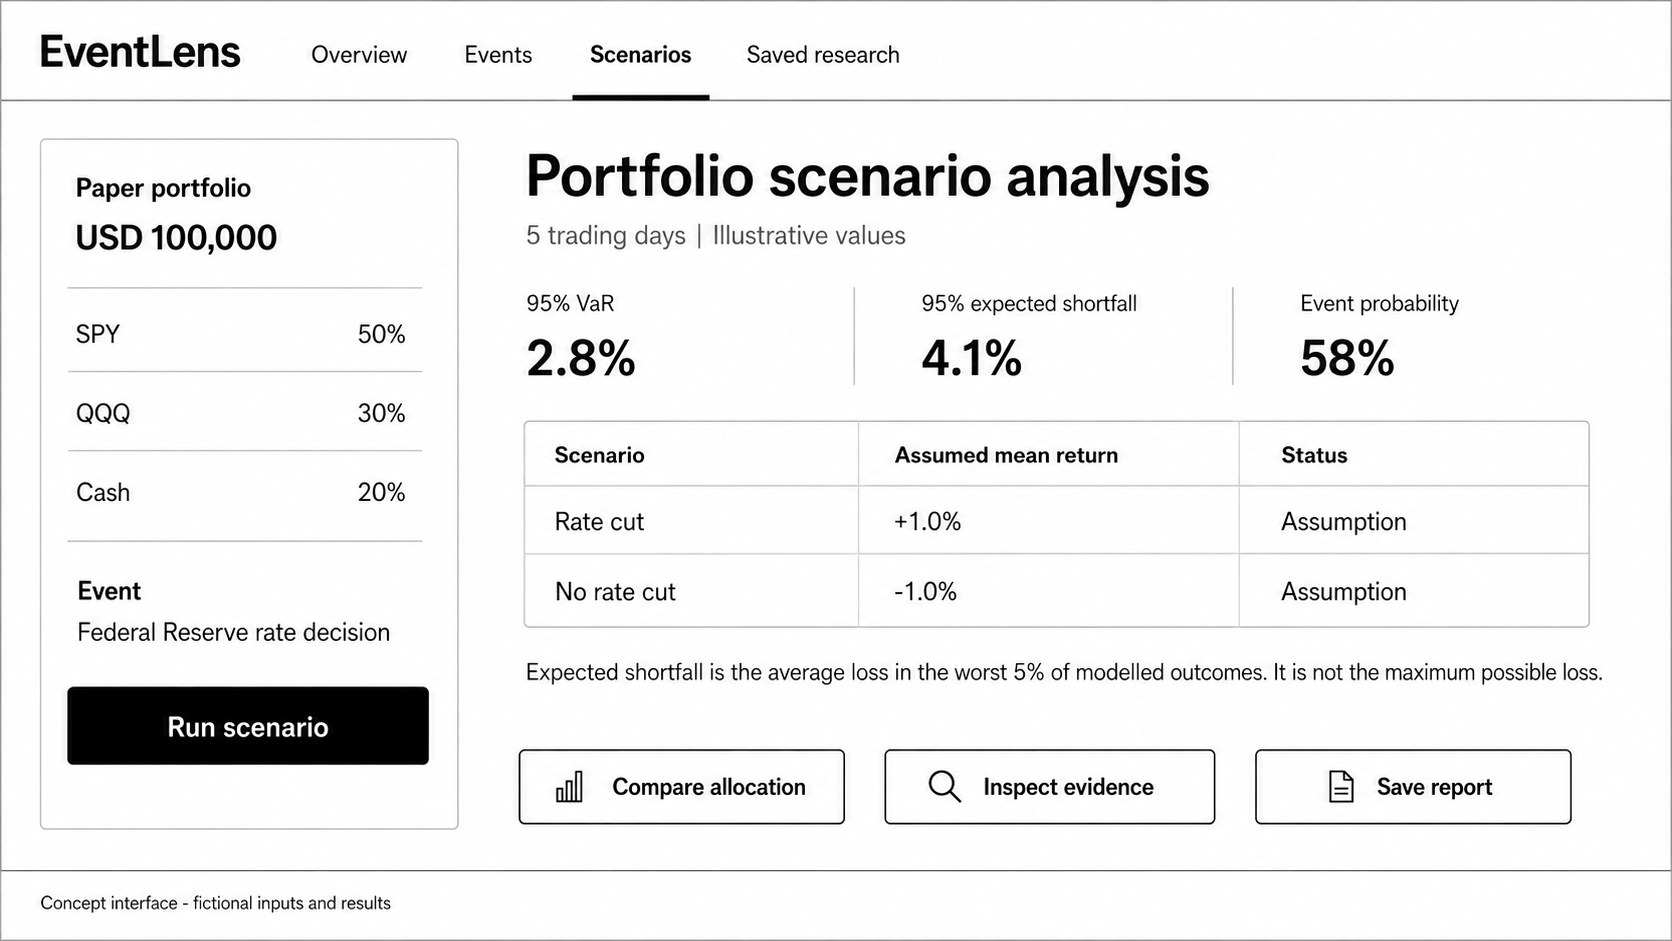
\includegraphics[width=\linewidth]{figures/scenario-ui.png}
\caption{\textbf{Scenarios} concept with a \textbf{Paper portfolio}, risk measures, assumptions and comparison actions. The user explores hypothetical results without placing orders.}
\label{fig:scenario-ui}
\end{figure}
